\documentclass[polish,12pt,a4paper]{extarticle}
\usepackage[T1]{fontenc}

\usepackage[top=2.5cm,bottom=2cm,left=2cm,right=2cm]{geometry}
\usepackage{xcolor}

\usepackage{placeins}  % in the preamble
\usepackage{babel}
\usepackage{titling}
\usepackage{lastpage}
\usepackage{amsmath}
\usepackage{amssymb}
\usepackage{stmaryrd}
\usepackage{fancyhdr}
\usepackage[bookmarks=false]{hyperref}
\usepackage{algorithm2e}
\usepackage{mathtools}
\usepackage{xcolor}
%\usepackage{overarrows}
\pagestyle{fancy}

\usepackage{tikz}
\usetikzlibrary{angles,quotes}

\title{Miniprojekt 2}
\author{Jakub Wieliczko}

\fancyhead[l]{MPUM}
\fancyhead[c]{\textbf{\thetitle}}
\fancyhead[r]{\theauthor}
\fancyfoot[c]{\begin{NoHyper}\thepage/\pageref{LastPage}\end{NoHyper}}

\newcommand{\inident}{\hspace{1.25em}}

% Algo stuff
\newcommand\mycommfont[1]{\ttfamily\textcolor{gray}{#1}}
\SetCommentSty{mycommfont}
\newcommand\Field[2]{\textbf{Field} $#1$: \texttt{#2}\;}
\newcommand\Method[3]{
	\SetKwFunction{Fn#1#2}{#1.#2}
	\SetKwFunction{FnLocal#1#2}{#2}
	\MethodImpl{\textnormal{\texttt{#2}(#3)}}
}
\newcommand\Struct[1]{
	\SetKwFunction{St#1}{#1}
	\StructImpl{\textnormal{\texttt{#1}}}
}

\newcommand\initalgorithm{
	\SetAlgoLined
	\DontPrintSemicolon
	\SetKwProg{Fn}{function}{:}{end}
	\SetKwProg{StructImpl}{struct}{:}{end}
	\SetKwProg{MethodImpl}{method}{:}{end}
}

% Math Stuff
\newcommand\Nat{\mathbb{N}}
\newcommand\Primes{\mathbb{P}}
\newcommand\eqqm[0]{\stackrel{?}{=}}
\renewcommand\lor{\,\vee\,}
\renewcommand\land{\,\wedge\,}
\newcommand\lxor[0]{\,\veebar\,}
\newcommand\union[0]{\cup}
\newcommand\isect[0]{\cap}
\newcommand\Union[0]{\bigcup}
\newcommand\Isect[0]{\bigcap}
\newcommand\nil[0]{\emptyset}
\renewcommand\geq{\geqslant}
\renewcommand\leq{\leqslant}
\newcommand\eqs[1]{\stackrel{#1}{=}}
\newcommand\impliesqm[0]{\stackrel{?}{\implies}}
\newcommand\QED[0]{\hfill$\blacksquare$}

\newcommand\set[1]{\left\{#1\right\}}
\newcommand\card[1]{\left|#1\right|}
\newcommand\cset[1]{\card{\set{#1}}}
\DeclarePairedDelimiter{\floor}{\lfloor}{\rfloor}
\DeclarePairedDelimiter{\ceil}{\lceil}{\rceil}

\newcommand{\stirC}[2]{\genfrac{[}{]}{0pt}{}{#1}{#2}}
\newcommand{\stirP}[2]{\genfrac{\{}{\}}{0pt}{}{#1}{#2}}


%\NewOverArrowCommand{image}{}
%\NewOverArrowCommand{coimage}{
%	end=\leftarrow
%}

\newcommand\stdarr[0]{\rightarrow}
\newcommand\injarr[0]{\hookrightarrow}
\newcommand\surarr[0]{\rightarrow\mathrel{\mspace{-15mu}}\rightarrow}
\newcommand\bijarr[0]{\hookrightarrow\mathrel{\mspace{-15mu}\rightarrow}}


\begin{document}


\begin{abstract}
    W poniższym dokumencie przedstawiam wnioski wyciągnięte podczas pisania projektu dot. klasyfikacji z Metod Probabilistycznych w Uczeniu Maszynowym. Celem projektu jest porównanie naiwnego klasyfikatora Bayesowskiego i regresji logistycznej.
\end{abstract}

\section*{Przygotowanie danych}
Na wejściu otrzymujemy zbiór danych postaci $D = \{(x^{(i)}_1, x^{(i)}_2, \dots, x^{(i)}_9, y^{(i)}): i = 1,2,\dots, m\}$, zatem mamy $9$ niezależnych cech opisujących badanie oraz informację, czy badany rak jest łagodny $(y = 2)$, czy złośliwy $(y = 4)$. Dla ułatwienia będę oznaczał $y = 2$ jako klasę $0$, zaś $y = 4$ jako klasę $1$ W celu podziału tych danych na zbiory treningowy i testowy, dzielę $D$ na $D_0$ i $D_1$ dla danych należących do klas odpowiednio $0$ i $1$, następnie dzielę obydwa zbiory w proporcji $2 : 1$ i łącząc te części tworzę zbiór treningowy $S$ i testowy $T$. W ten sposób losowo wybrana dana z $S$ ma takie same prawdopodobieństwo bycia w klasie $0$, co losowo wybrana dana z $T$.
\section*{Wstępna analiza danych}
Każda z cech jest pewną liczbą całkowitą ze zbioru $\{1, 2, \dots, 10\}$. Dla naszych danych nie stosuję standaryzacji, gdyż przy \textbf{naiwnym klasyfikatorze bayesowskim} standaryzacja danych które chcemy podzielić na klasy i tak nie miałaby sensu, a dla \textbf{regresji logistycznej} zakresy tych danych są na tyle małe, że nie utrudnia wyboru współczynnika \texttt{learning rate}, ani nie psuje regularyzacji. Popatrzmy teraz na rozkład poszczególnych cech.
\begin{figure}[h!]
    \centering
    \begin{minipage}[b]{0.3\textwidth}
    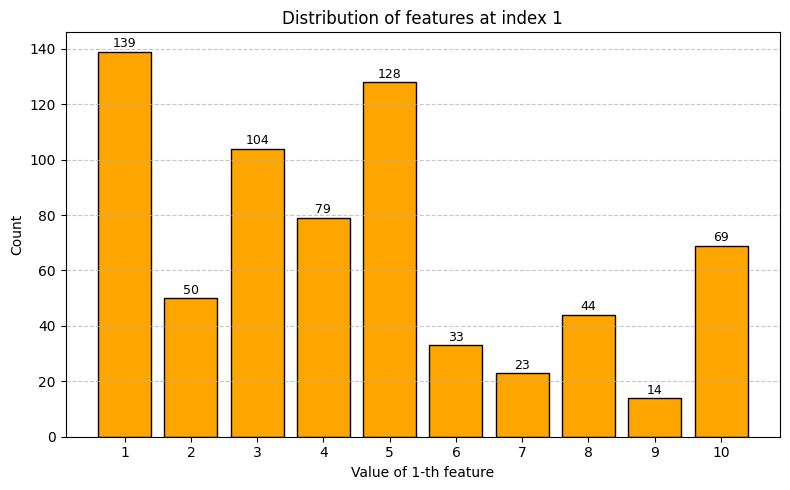
\includegraphics[width=0.9\textwidth]{img/feature_1.png}
    \end{minipage} \hspace{}
    \begin{minipage}[b]{0.3\textwidth}
    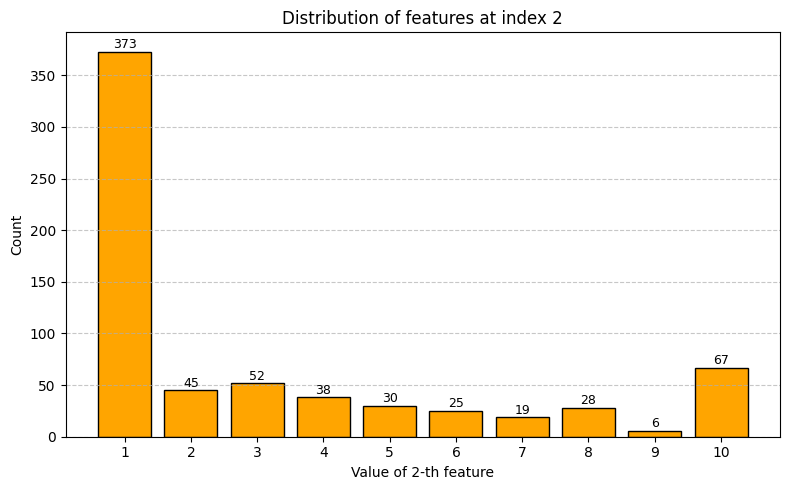
\includegraphics[width=0.9\textwidth]{img/feature_2.png}
    \end{minipage} \hspace{}
    \begin{minipage}[b]{0.3\textwidth}
    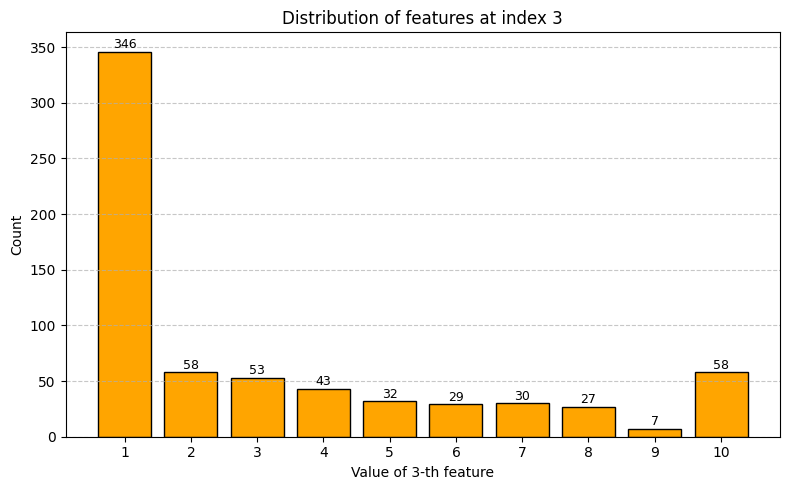
\includegraphics[width=0.9\textwidth]{img/feature_3.png}
    \end{minipage}
\end{figure} \smallskip \\
\begin{figure}[h!]
    \centering
    \begin{minipage}[b]{0.3\textwidth}
    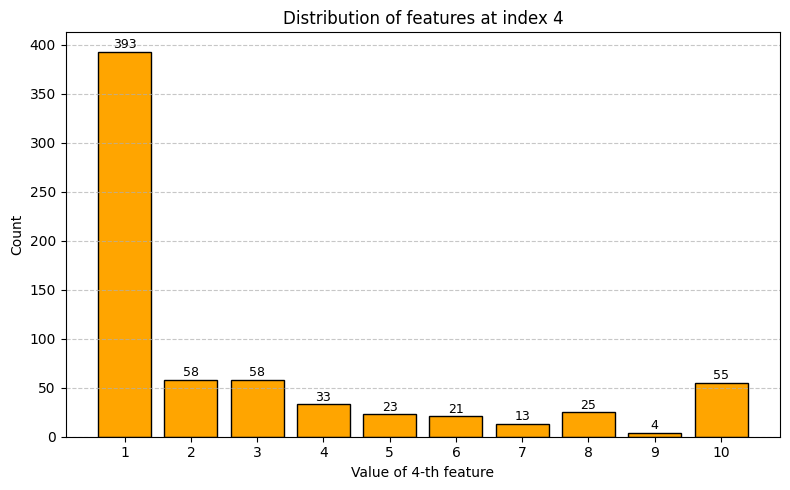
\includegraphics[width=0.9\textwidth]{img/feature_4.png}
    \end{minipage} \hspace{}
    \begin{minipage}[b]{0.3\textwidth}
    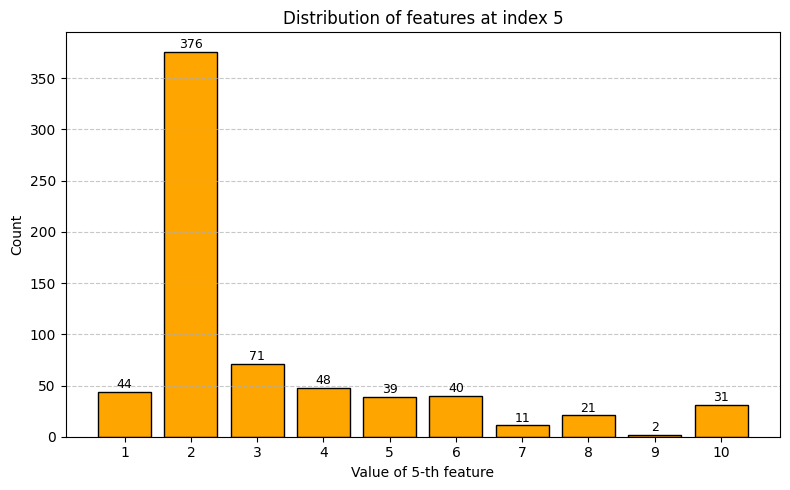
\includegraphics[width=0.9\textwidth]{img/feature_5.png}
    \end{minipage} \hspace{}
    \begin{minipage}[b]{0.3\textwidth}
    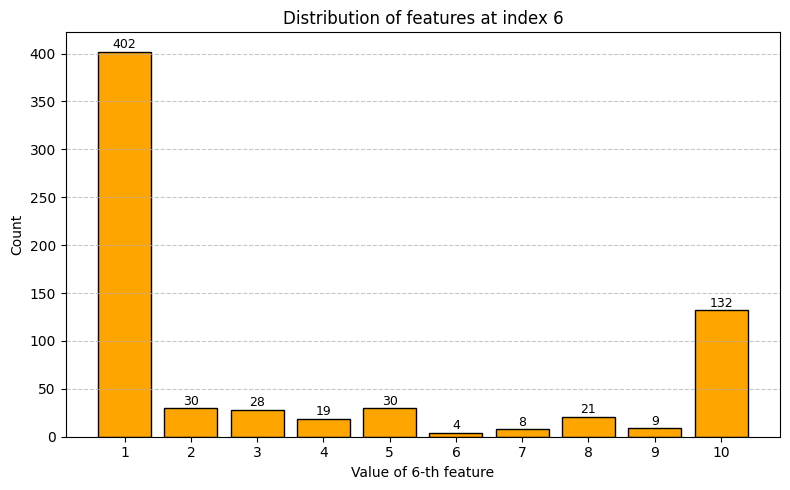
\includegraphics[width=0.9\textwidth]{img/feature_6.png}
    \end{minipage}
\end{figure} \smallskip \\
\begin{figure}[h!]
    \centering
    \begin{minipage}[b]{0.3\textwidth}
    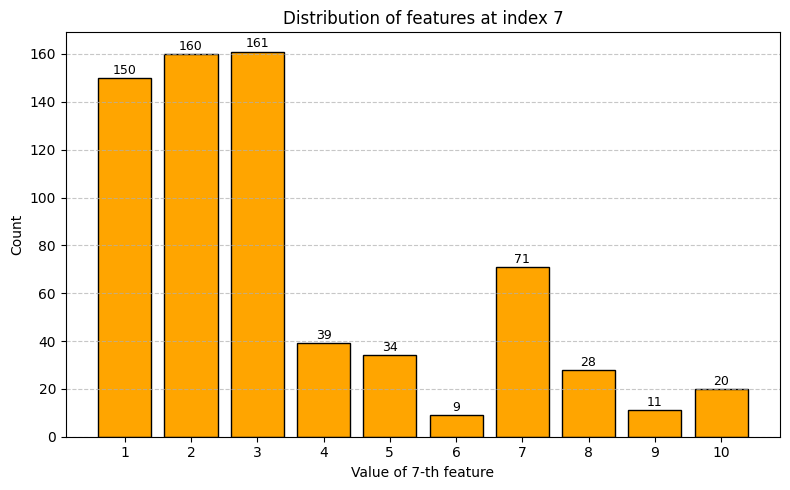
\includegraphics[width=0.9\textwidth]{img/feature_7.png}
    \end{minipage} \hspace{}
    \begin{minipage}[b]{0.3\textwidth}
    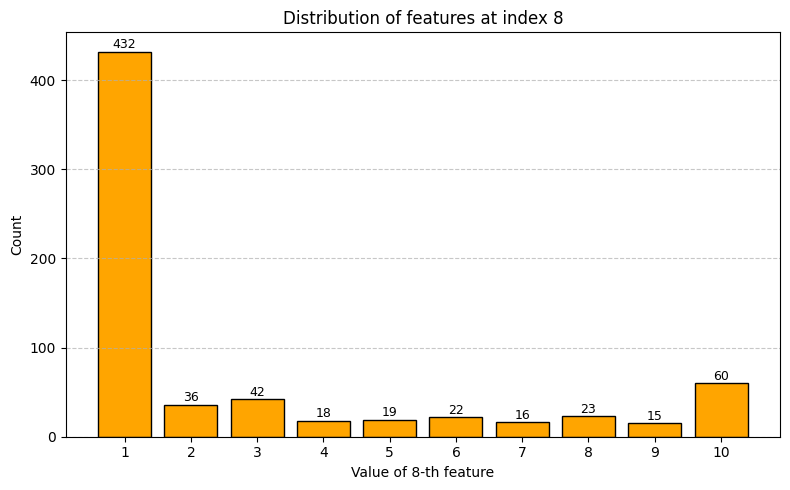
\includegraphics[width=0.9\textwidth]{img/feature_8.png}
    \end{minipage} \hspace{}
    \begin{minipage}[b]{0.3\textwidth}
    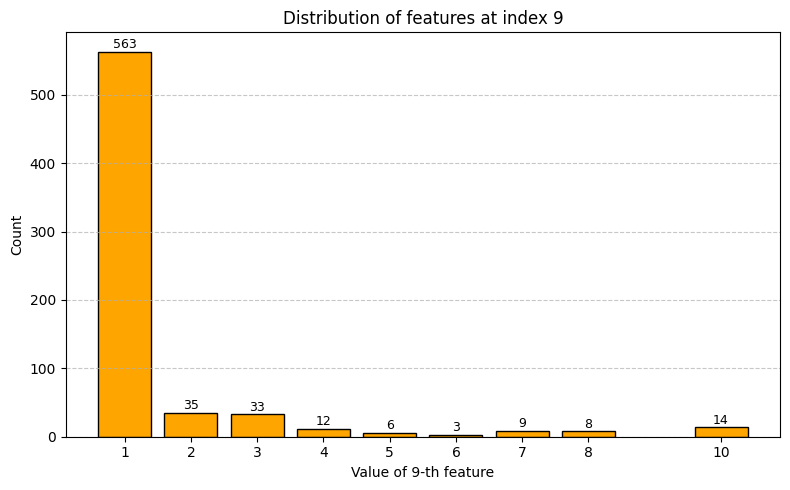
\includegraphics[width=0.9\textwidth]{img/feature_9.png}
    \end{minipage}
\end{figure} \FloatBarrier
Widzimy, że w niektórych przypadkach cechy mają wartość wokół której się koncentrują, a w innych występują równomiernie różne ich wartości.
\section*{Ocena skuteczności modeli}
Sposób w jaki sprawdzam skuteczność modeli jest następujący: najpierw trenuję model na zbiorze treningowym, a następnie tak obliczone parametry używam do klasyfikacji danych ze zbioru testowego. Następnie porównuję przewidywania z faktycznymi wynikami na zbiorze testowym i liczę ile jest przypadków \texttt{True Positive}, \texttt{False Positive}, \texttt{True Negative} oraz \texttt{False Negative}. Na ich podstawie wyliczam statystyki, takie jak precyzja i czułość. \smallskip \\
Miarą, której używam do oceny klasyfikatorów to miara $F_1$, gdyż zależy mi obecnie na modelu który zarówno wykrywa jak najwięcej przypadków i przy okazji unika fałszywych alarmów. \begin{center}
$F_1(\mathrm{precision}, \mathrm{sensitivity}) = \frac{2 \cdot \mathrm{precision} \cdot \mathrm{sensitivity}}{\mathrm{precision} + \mathrm{sensitivity}}$
\end{center}
Możemy teraz przejść do porównania wyników obydwu modeli.

\section*{Regresja logistyczna}
Na potrzeby tego projektu zaimplementowałem regresję logistyczną używając do tego klayscznego algorytmu spadku wzdłuż gradientu. Nie zdecydowałem się na żadne optymalizacje, np. \textbf{mini$-$batch}, gdyż model trenował się względnie bardzo szybko: dla $n = 15000$ iteracji (dla tylu epok wyniki już były satysfakcjonujące), na pełnym zbiorze treningowym przebieg algorytmu zajmował ok. $5$ sekund. Za \texttt{learning rate} wziąłem współczynnik $\eta = 0.0025$ \smallskip \\
Do regresji logistycznej wykorzystałem następującą \texttt{funkcję błędu} z wykorzystaniem regularyzacji $L_2$:
\begin{center}
    $L(\theta) = \frac{-1}{m}\sum_{i=1}^m (1 - y^{(i)}) \cdot \ln(1 - h_{\theta}(x^{(i)})) + (y^{(i)}) \cdot \ln(h_{\theta}(x^{(i)})) + \lambda \cdot \theta^T \theta $
\end{center}
Gdzie za naszą hipotezę bierzemy funkcję sigmoid
\begin{center}
    $h_{\theta}(x) = \sigma(\theta^Tx)$
\end{center}
Licząc pochodne cząstkowe, dostajemy
\begin{center}
    $\frac{\partial}{\partial \theta_j} L(\theta) = \frac{1}{m}\sum_{i=1}^m (h_{\theta}(x^{(i)}) - y^{(i)}) x_j^{(i)} + 2\lambda \cdot \theta_j$
\end{center}
Na poniższym wykresie przedstawiam zależność funkcji straty od liczby iteracji. \\
\begin{figure}[h!]
    \centering
    \begin{minipage}[b]{0.35\textwidth}
    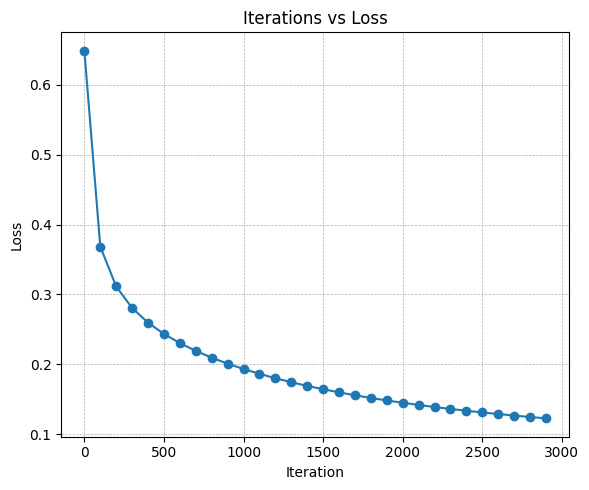
\includegraphics[width=0.7\textwidth]{img/it_loss_small.png}
    \caption{$n = 3000$ iteracji}
    \end{minipage} \hspace{}
    \begin{minipage}[b]{0.35\textwidth}
    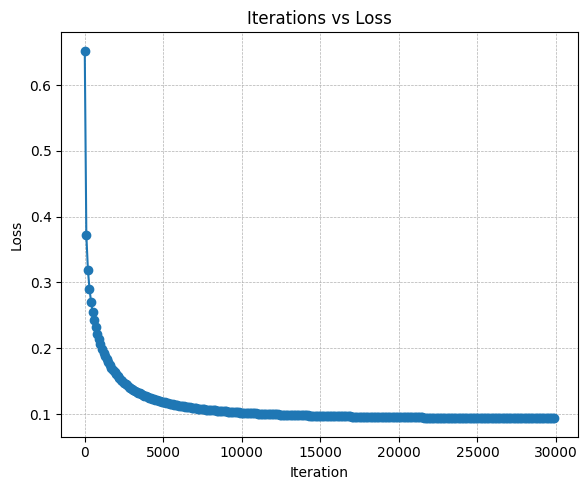
\includegraphics[width=0.7\textwidth]{img/it_loss_big.png}
    \caption{$n = 30000$ iteracji}
    \end{minipage}
\end{figure} \smallskip \\ \FloatBarrier
Tempo malenia funkcji straty jest nieporównywalnie mniejsze gdy rozważamy duże iteracje, więc stwierdziłem że wystarczy trenować model do $n = 15000$ iteracji. Warto nadmienić, że $3000$ iteracji zajęło mi ok. $1.66s$, a $30000$ iteracji ok. $16.1s$. \bigskip \\
Kolejnym aspektem, nad którym się chciałbym pochylić, to jak regularyzacja wpływa na wynik naszego modelu na testowym zbiorze danych. W tym projekcie używam regularyzacji grzbietowej. Nie korzystam ze zbioru walidacyjnego, zatem to w jaki sposób zmierzę współczynnik $\lambda$ to przez uśrednianie wyniku mojego algorytmu na kilku podziałach danych na zbiory treningowy i testowy. Porównanie różnych wspołczynników regularyzacji $\lambda$ przedstawia się następująco. \smallskip \\
\begin{figure}[h!]
    \centering
    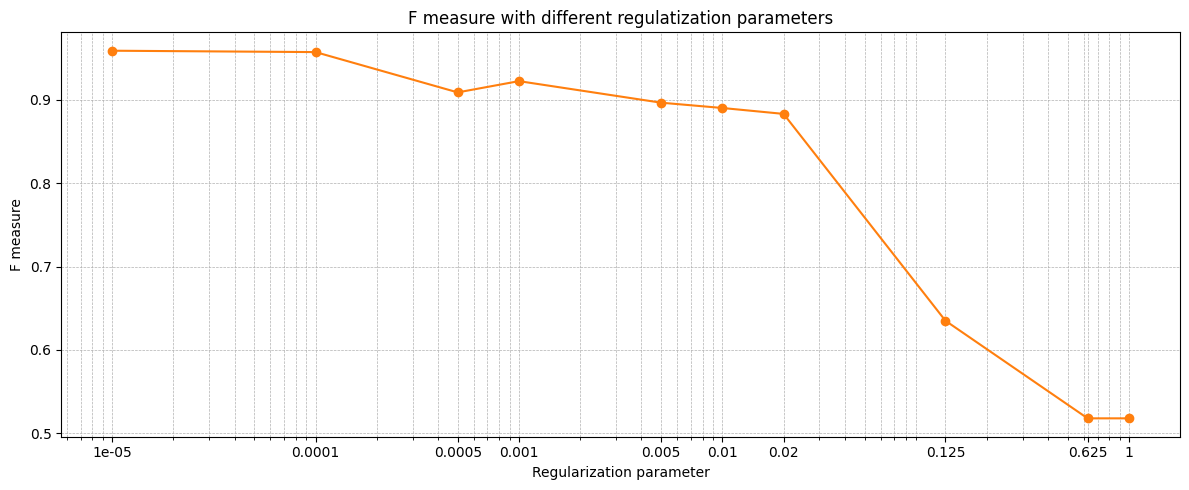
\includegraphics[width=0.65\textwidth]{img/reg_f.png}
    \caption{Miara $F_1$ dla różnych wyborów współczynnika $\lambda$}
\end{figure}
\begin{figure}[h!]
    \centering
    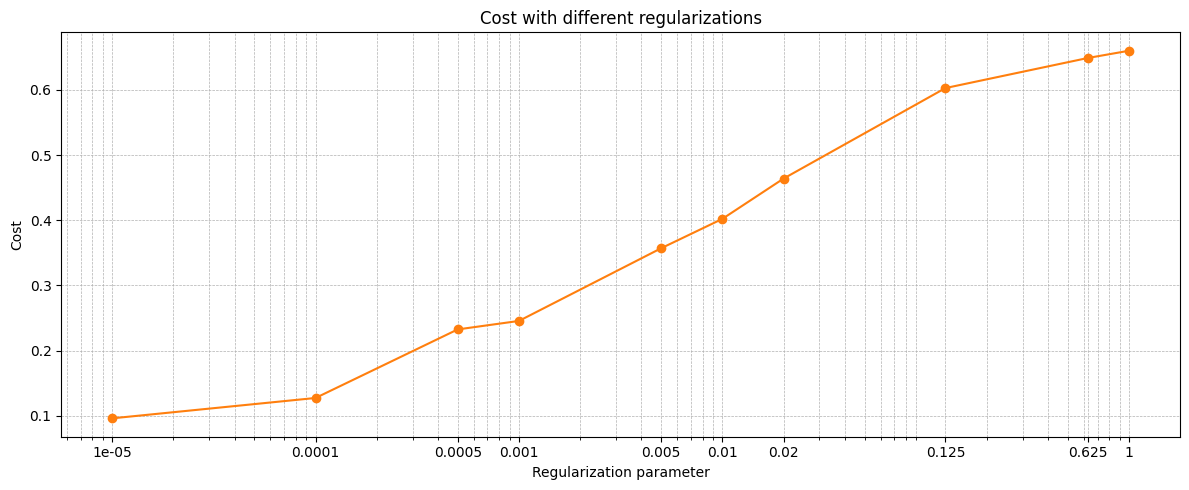
\includegraphics[width=0.65\textwidth]{img/reg_cost.png}
    \caption{Błąd $L$ na zbiorze testowym obliczony dla różnych wyborów współczynnika $\lambda$} \end{figure} \FloatBarrier
Jak widać, model nie overfituje się na zbiorze treningowym i regularyzacja nie poprawia wyników naszego modelu. Wraz ze wzrostem parametru błąd też znacząco rośnie, zatem algorytm zamiast "wygładzać" funkcję, koncentruje się na minimalizacji współczynników przez co algorytm nie osiąga lepszych efektów. Przez to że regularyzacja nie poprawia wyników naszego modelu, w końcowym porównaniu nie będę jej stosował. \smallskip \\
Biorąc wcześniejsze wnioski pod uwagę, zmierzmy teraz kilka parametrów trenując nasz model na pełnym zbiorze treningowym. Wyniki które otrzymałem są następujące.
\begin{table}[h!]
\centering
\begin{tabular}{|l|c|}
\hline
\textbf{Parametr}       & \textbf{Wartość} \\
\hline
Dokładność              & 0.987          \\
Precyzja             & 0.975          \\
Czułość           & 0.987          \\
Swoistość           & 0.986          \\
Miara F             & 0.981          \\
\hline
\end{tabular}
\caption{Wyniki najlepszego modelu}
\label{tab:performance_metrics}
\end{table} \FloatBarrier

\section*{Naiwny klasyfikator Bayesowski}
Przejdźmy teraz do generatywnego algorytmu klasyfikacji. W tym projekcie zaimplementowałem \texttt{naiwny klasyfikator Bayesowski} z wykorzystaniem \texttt{wygładzenia Laplace'a}. W tym celu dla danych treningowych $T$ liczę następujące parametry:
\begin{center}
    $\Phi_y = \frac{1 + \sum_{i=1}^m \mathbf{1}[y^{(i)} = 1]}{2 + m}$
\end{center}
\begin{center}
    $\Phi_{c, d}^j = \frac{1 + \sum_{i=1}^m \mathbf{1}[y^{(i)} = c \, \wedge \, x^{(i)}_j = d]}{10 + \sum_{i=1}^m \mathbf{1}[y^{(i)} = c]}$
\end{center}
Pierwszą rzeczą, na którą zwróciłem uwagę, była szybkość tego algorytmu. Wytrenowanie modelu na pełnym zbiorze treningowym zajmowało mi ok. $10$ ms, co było nieporównywalnie szybsze względem regresji logistycznej. \smallskip \\
Ciekawą rzeczą, którą zauważyłem analizując proces trenowania naiwnego klasyfikatora bayesowskiego, było to że gdy używałem więcej niż $12.5\%$ zbioru treningowego to im więcej miał danych, tym bardziej pewne decyzje na zbiorze testowym podejmował. Zatem zdecydowaną część wyników szacował albo na $0.00\%$, albo na $99.99\%$ (decyzje były \textit{troszeczkę} bardziej zrównoważone gdy użyłem \texttt{log-prawdopodobieństwa}, ale odpowiedzi nadal były, delikatnie rzecz ujmując, \textbf{stanowcze}). \smallskip \\
Poniżej przedstawiam uśrednione wyniki, jakie udało mi się osiągnąć używając \textbf{naiwnego klasyfikatora Bayesowskiego}. \\
\begin{table}[h!]
\centering
\begin{tabular}{|l|c|}
\hline
\textbf{Parametr}       & \textbf{Wartość} \\
\hline
Dokładność              & 0.978          \\
Precyzja             & 0.963          \\
Czułość           & 0.975          \\
Swoistość           & 0.980          \\
Miara F             & 0.969          \\
\hline
\end{tabular}
\caption{Wyniki najlepszego modelu}
\label{tab:performance_metrics}
\end{table} \FloatBarrier
Zauważmy, że są one równie wysokie co dla algorytmu \textbf{regresji logistycznej}, mimo naszego silnego założenia że cechy są warunkowo niezależne.
\section*{Trenowanie na frakcjach zbioru treningowego}
Pytanie na które chciałbym odpowiedzieć, to ile danych wystarczy żeby satysfakcjonująco wytrenować klasyfikator. W tym celu wytrenowałem obydwa modele na różnych frakcjach zbioru treningowego, a wyniki znajdują się poniżej.
\begin{figure}[h!]
    \centering
    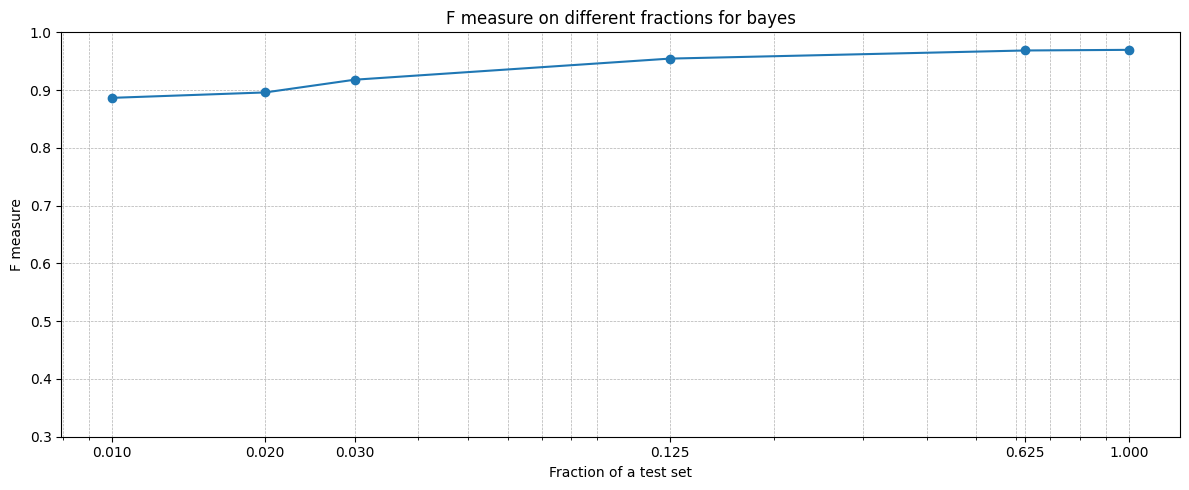
\includegraphics[width=0.65\textwidth]{img/bayes_frac_better.png}
    \caption{Miara $F_1$ dla frakcji przy uczeniu naiwnego klasyfikatora Bayesowskiego}
\end{figure} \\
\begin{figure}[h!]
    \centering
    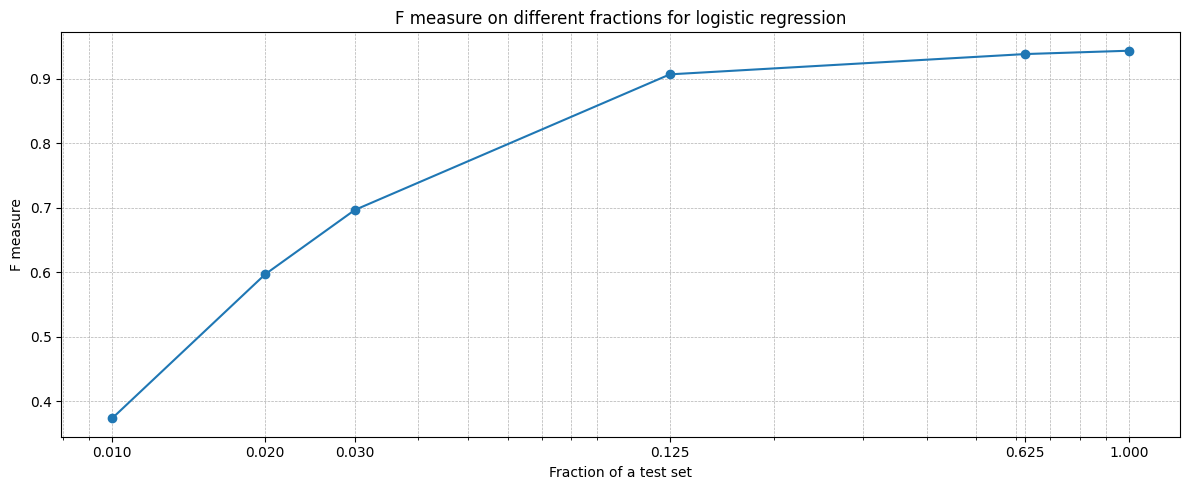
\includegraphics[width=0.65\textwidth]{img/logistic_frac.png}
    \caption{Miara $F_1$ dla frakcji przy uczeniu algorytmem regresji logistycznej}
\end{figure} \\
Od początku widzimy bardzo dużą różnicę. Otóż, gdy popatrzymy na skalę miary $F_1$, naiwny klasyfikator bayesowski od początku radzi sobie dużo lepiej, przy czym już $1\%$ zbioru treningowego pozwala mu na nauczenie się danych na tyle dobrze, żeby otrzymywać średnio miarę $0.89$. Jest to wynik do którego regresja logistyczna zbliża się dopiero przy $12.5\%$ zbioru treningowego, a nasz klasyfikator Bayesowski otrzymuje już miary rzędu $0.94$
\section*{Wnioski}
Według autora artykułu powszechnie uważa się modele dyskryminatywne za dokładniejsze od modeli generatywnych. W przypadku naiwnej klasyfikacji Bayesowskiej bardzo silnym założeniem jest warunkowa niezależność cech, taki model nie bierze tych zależności pod uwagę. Jednak w naszym przypadku obydwa modele osiągnęły bardzo satysfakcjonujące wyniki. Teza płynąca z artykułu to fakt, że \texttt{naiwny klasyfikator Bayesowski} potrafi się uczyć już na bardzo małej ilości danych (mowa jest o rozmiarze danych rzędu $O(\log n)$ i rzeczywiście, naiwny klasyfikator Bayesowski osiąga nienajgorszy wynik biorąc jedynie $1\%$ danych treningowych.
\end{document}
